% Tropical character sheet by French Rice Merman

\documentclass[12pt]{article}
\usepackage{charsheet}
\usepackage{multicol}
\usepackage{amsmath}
\usetikzlibrary{fit}
%\usepackage{amsmath}
\colorlet{grayed out}{white!70!black}

\newcommand\scrm[1]{\textrm{\textsc{#1}}}

\newcommand\bigstrut{\vrule width 0pt height 16pt depth 0pt }

\usepackage{pgfkeys}

% Incomplete character support

\newcommand\fillin[1]{%
  \hbox{\vrule height 0pt depth 0.8pt width #1}%
}


\newdimen\textmargin % amount subtracted from each side to get `text width`
\textmargin=8pt

\newdimen\mynodedistance
\mynodedistance=7pt

\tikzset{%
  minimum label sep=6pt,
  every label node part/.style={
     text width=,
     font=\sffamily\footnotesize,
  },
  widecolumn/.style={
    labeled decorated stub rectangle,
    text width=134mm-2\textmargin,
    inner xsep=8pt,
    align=justify,
    font={\rightskip=0pt plus 2em},
    inner ysep=6pt,
    outer xsep=0pt, % x placement is happening by hand
    draw, line width=1.2pt,
    stub radius=2.3mm,
  },
  narrowcolumn/.style={
    widecolumn,
    text width=36mm-2\textmargin,
  },
  initiative/.style={
    labeled decorated clipped rectangle,
%    minimum width=\hpwidth/3-10pt,
    draw, line width=1.2pt,
    fill=white,
%    yseparated,
    outer xsep=3pt,
    minimum height=17mm,
  },
  dnd hit dice/.style={
    dnd max hp,
%    labeled decorated clipped rectangle,
%    yseparated,
%    minimum width=\hpwidth/2-5pt,
    minimum height=18mm,
    font=\footnotesize,
  }
}

  
\newenvironment{merman attacks}
  {\begin{minipage}{\linewidth}
   \raggedright
   \scriptsize
   \let\dndkeys=\mermanattackkeys
  }
  {\par\end{minipage}}

\makeatletter
\newcommand\mermanattackkeys[1]{%
  \gdef\@attackname{}%
  \gdef\@attackattack{}%
  \gdef\@attackdamage{}%
  \gdef\@attacktype{}%
  \gdef\@attackrange{}%
  \gdef\@attackammotype{}%
  \gdef\@attackammocount{}%
%  {\def\statdc{\protect\statdc}\typeout{attack keys: #1}}%
  \pgfkeys{/attacks/.cd, #1}%
  \hangindent=2em \hangafter=1
  \@attackname~\signed{\@attackattack}, \@attackdamage~\@attacktype (\@attackrange)\par
}
\makeatother




\newcommand\fboxzero[1]{{\fboxsep=0pt \fbox{#1}}}


\begin{document}




\input{stats}

\noindent
\begin{charsheet}[x=1mm,y=1mm,inner sep=0pt]
  \tikzset{node distance=\mynodedistance}

\node [anchor=south west] (merman) at (0,0) {
   \vbox{
    \vspace*{15mm}
   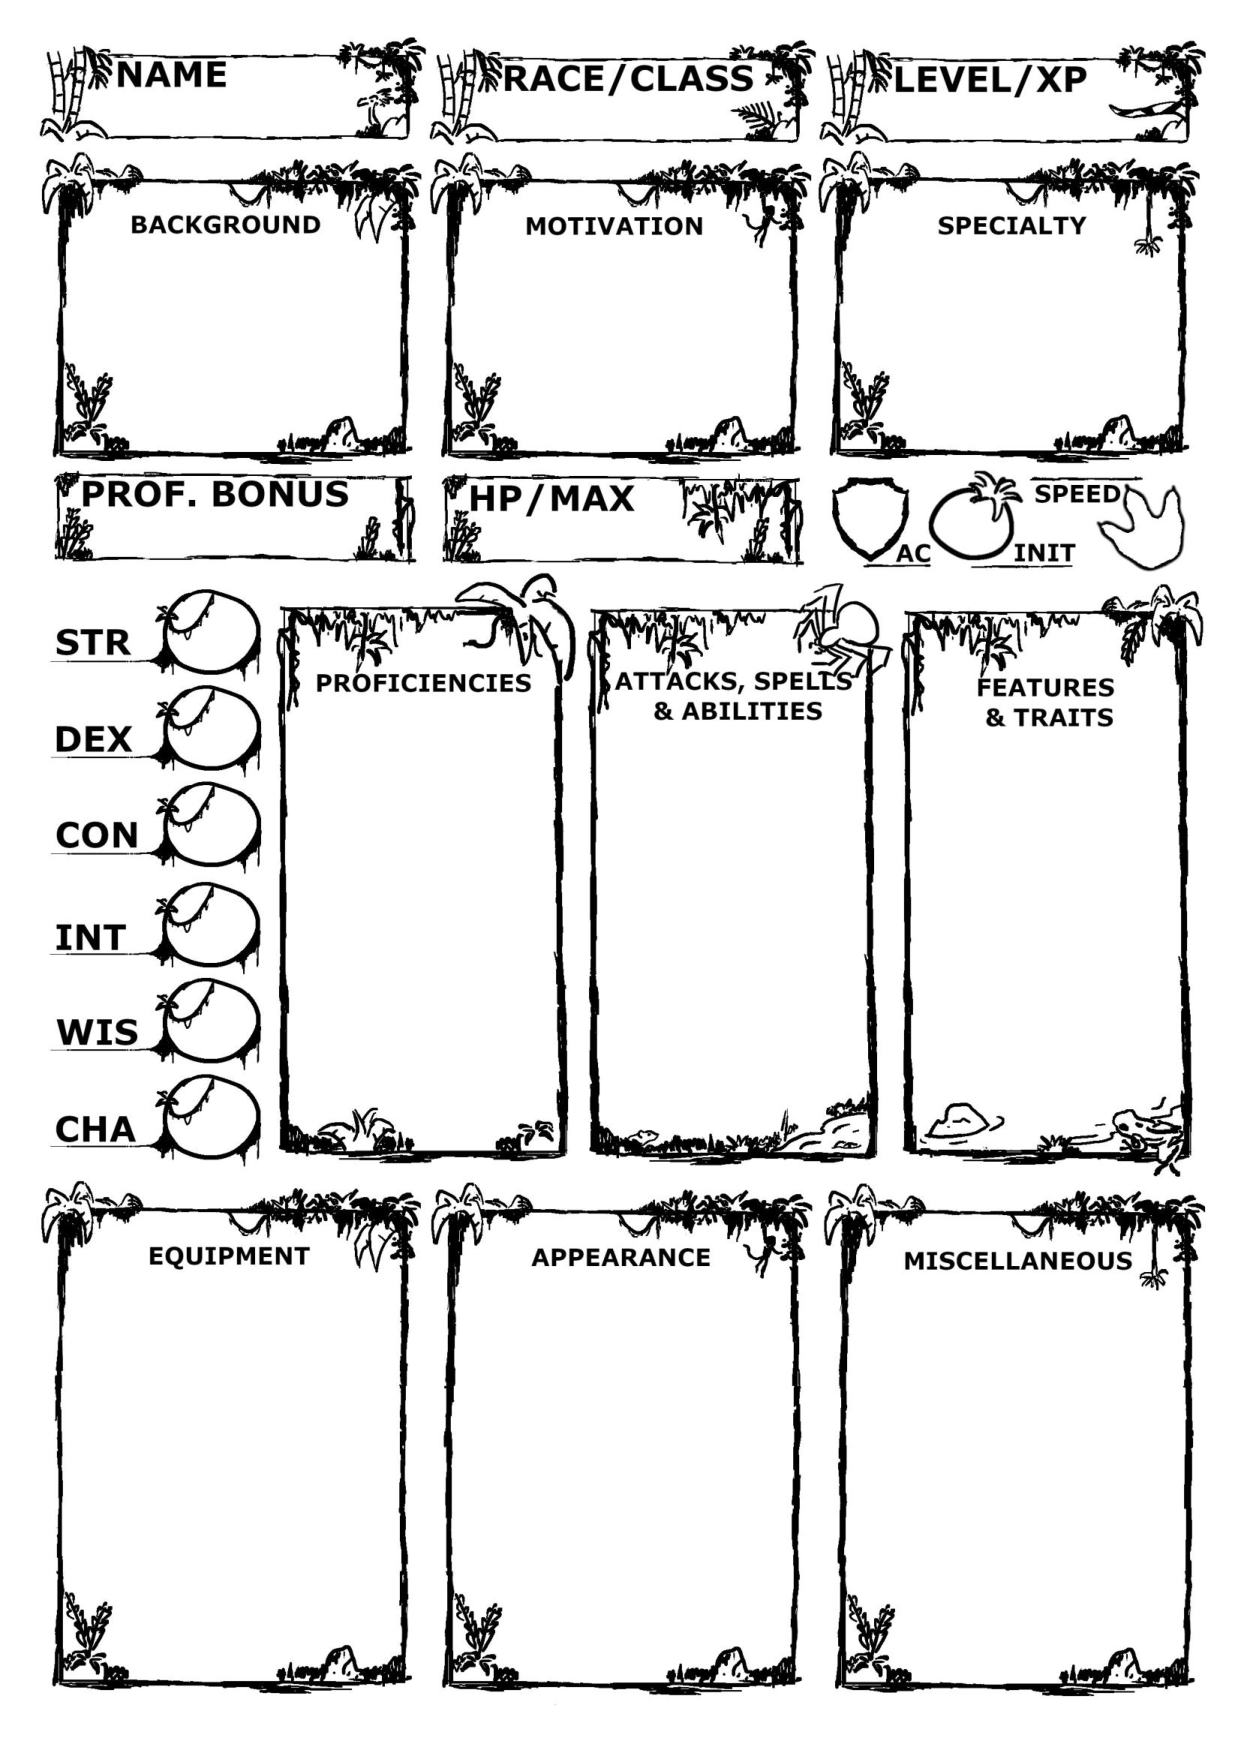
\includegraphics[height=\paperheight]{merman.pdf}
    \vspace*{-15mm}
   }
};

\path [opacity=0.57,fill=white] (merman.south west) rectangle (merman.north east);

% Grid overlay: thin line every 1mm, heavy every 10mm, labels every 10mm.
% Grid is anchored to the image's SW corner so labels align with gridlines.
% NB: charsheet env uses x=1cm,y=1cm, so step must be given with explicit mm
% units (otherwise step=1 means 1cm and the thin grid coincides with the heavy).

\iffalse

    \begin{scope}
      \clip (merman.south west) rectangle (merman.north east);
      \draw[blue!40, line width=0.1pt]
        (merman.south west) grid[step=1mm] (merman.north east);
      \draw[blue!60, line width=0.8pt]
        (merman.south west) grid[step=10mm] (merman.north east);
      \foreach \x in {0,10,...,300} {
        \node[anchor=south west, font=\tiny\sffamily\bfseries,
              text=blue, inner sep=1pt]
          at ([xshift=\x mm]merman.south west) {\x};
      }
      \foreach \x in {0,10,...,300} {
        \path ([xshift=\x mm]merman.south west) ++(0,180mm) 
           node [anchor=north west, font=\tiny\sffamily\bfseries,
                 text=blue, inner sep=1pt]
           {\x}
           ;
      }
      \foreach \y in {10,20,...,300} {
        \node[anchor=south west, font=\tiny\sffamily\bfseries,
              text=blue, inner sep=1pt]
          at ([yshift=\y mm]merman.south west) {\y};
      }
    \end{scope}

\fi


\LARGE
\sffamily
\bfseries
\color{blue!60!black}

\path (41,169.5) node (STR)  {\dndmodifier{STR}}
    ++(0, -15.5)  node (DEX) {\dndmodifier{DEX}}
    ++(0, -15.5)  node (CON) {\dndmodifier{CON}}
    ++(0, -15.7)  node (INT) {\dndmodifier{INT}}
    ++(0, -15.5)  node (WIS) {\dndmodifier{WIS}}
    ++(0, -15.5)  node (CHA) {\dndmodifier{CHA}}
;


\begin{scope}
\large
\tikzset{anchor=north}

\path (21,163) node (STR)  {\getDND*{STR}}
    ++(0, -15.5)  node (DEX) {\getDND*{DEX}}
    ++(0, -15.5)  node (CON) {\getDND*{CON}}
    ++(0, -15.7)  node (INT) {\getDND*{INT}}
    ++(0, -15.5)  node (WIS) {\getDND*{WIS}}
    ++(0, -15.5)  node (CHA) {\getDND*{CHA}}
;

\end{scope}

\normalsize

\path (168,0) coordinate (right center);
\path (44,0) coordinate (left center);
\path (105,0) coordinate (center);

\path(0,250) coordinate (top baseline);

\begin{scope}
\tikzset{anchor=south}
\node [anchor=south] (race/class) at (top baseline -| left center) {\getDND*{CHARACTER NAME}};

\node [anchor=south] (race/class) at (top baseline -| center) {\getDND*{RACE}/\getDND*{CLASS}};

\node [anchor=south] (level/xp) at (top baseline -| right center)
         {\getDND*{LEVEL} / \fillin{1in}}
  ;

\path (0,183) coordinate (hp baseline);

 \node [anchor=south] (proficiency bonus) at (left center |- hp baseline)
       {+\arabic{proficiency bonus}}
    ;

\node [anchor=south] (hp/max) at (center |- hp baseline)
 {\fillin{2cm} / \getDND*{MAX HP}\hspace*{1cm}};

\path (hp baseline) ++(0,2) coordinate (ac baseline);

\path (144.5,0 |- ac baseline) ++(0,1) node {\large\getDND*{ARMOR CLASS}};

\path (161.0,0 |- ac baseline) ++(0,-0.5) node {\whenDNDdefined{INITIATIVE}{\signed{\rawgetDND{INITIATIVE}}}};

\path (189.7,0 |- hp baseline) ++(0,-1) node {\getDND*{SPEED}};

\tikzset{anchor=north}

\path (0, 230) coordinate (bg top);

\node [anchor=north] (background) at (bg top -| left center) {\getDND*{BACKGROUND}};

\node (motivation) at (bg top -| center)
      {\begin{minipage}{4cm}\centering\getDND*{MOTIVATION}\end{minipage}};


\end{scope}

 \node (proficiencies)
     [text width=4.2cm,
      anchor=north,
     ]
   at (72, 160)
  { \useDNDfont*{PROFICIENCIES}
    \newif\ifprofs
    \scriptsize
    \profsfalse
    \whenDNDnonempty{PROFICIENCIES}\profstrue
%    \whenDNDnonempty{SECONDARY PROFICIENCIES}\profstrue
    \begin{proflist}
    \let\profskip=\smallskip
    \raggedright
    \getDND*{PROFICIENCIES}
%    \whenDNDnonempty{PROFICIENCIES}{%
%        \whenDNDnonempty{SECONDARY PROFICIENCIES}{\profskip}}
%    \getDND*{SECONDARY PROFICIENCIES}
    \relax
    \ifprofs\else \item (No proficiencies listed.)\fi
    \end{proflist}
  }
;



\node (attacks etc) [anchor=north, text width=4.3cm] at (124, 153)
     {
     \centering
     \useDNDfont*{ATTACKS}
     \noindent
    \let\small=\tiny
     \begin{merman attacks}
     \gdef\notesheader{\cline{2-4}}%
     \gdef\notesheader{}%
     \gdef\attacknote#1#2{}%  Just don't
     \getDND{ATTACKS}%

     \whenDNDdefined{MAGIC}
     {
      \par\smallskip
      \advance\baselineskip by 2pt \selectfont
      \def\spellslevellabel#1#2{\ignorespaces\relax}%
      \def\describedColored#1#2#3{\emph{#2}\\}%
      \def\described#1#2{\emph{#1}\\}%
      \rawgetDND{MAGIC}%
     }
     \end{merman attacks}
  }
  ;
  

  \whenDNDdefined{FEATURES}{
      \node[text width=4.3cm, anchor=north] 
       (features)
        at (173, 0 |- attacks etc.north)
       {\def\described#1#2{%
           \hangindent=2em \hangafter=1
           \scriptsize #1: \tiny #2 \par
        }
        \def\describedColored#1{\described}%
        \begin{merman attacks}
        \parskip=2.5pt
        \let\rlapequip\relax
        \getDND{FEATURES}
        \end{merman attacks}
       };
  }

\path (right center) coordinate (bottom right center);
\path (42,0) coordinate (bottom left center);
\path (center) coordinate (bottom center);

\path (0, 68) coordinate (equipment top);

  \whenDNDdefined{EQUIPMENT}{%
      \node[text width=4.3cm, anchor=north] 
       (equipment)
        at (bottom left center |- equipment top)
        {
          \begin{minipage}{\linewidth}
          \scriptsize
          \begin{eqlist}%
         \ifDNDnonempty{EQUIPMENT}
            {\getDND{EQUIPMENT}}
            {\item (Placeholder: Equipment will go here.)}%
         \end{eqlist}
         \end{minipage}%
       }
      ;
  }


%%%%      \node (equipment) [draw=none,fill=none,left of lower corner=of features] {};
%%%%    }
%%%%    
%%%%    \path (equipment.north west) +(3mm,-\mynodedistance) coordinate (coin top left);
%%%%    
%%%%    \coin{cp}{Cu}{\color{grayed out}\getDND*{CP}}
%%%%    \coin{sp}{Ag}{\color{grayed out}\getDND*{SP}}
%%%%    \coin{gp}{Au}{\color{grayed out}\getDND*{GP}}
%%%%    \coin{pp}{Pt}{\color{grayed out}\getDND*{PP}}
%%%%      
%%%%    \setdeltax\sectionwidth{attacks.west}{stats background.east}
%%%%    \path (stats background.east) ++(\mynodedistance,0) ++(-2.5pt,0) coordinate (prof circle west);
%%%%    \node (proficiency circle) [anchor=west,proficiencies,circle,
%%%%           width=10mm,height=10mm,line width=1.5pt,draw]
%%%%           at (prof circle west |- proficiency bonus.center)
%%%%          {\large\textsf{+\arabic{proficiency bonus}}};
%%%%    
%%%%    \draw [line width=0.5pt] (proficiency circle) circle [radius=4.2mm];
%%%%    
%%%%    % center the text in the visible space
%%%%    \setdeltax\tmpwidth{proficiency bonus.east}{proficiency circle.east}
%%%%    
%%%%    % proficiencies bottom should be stats background bottom or equipment
%%%%    % top, whatever is higher
%%%%    
%%%%    
%%%%      \setdeltay\tmpheight{stats background.south}{equipment.north}
%%%%      \advance\tmpheight by -\mynodedistance % allows space above equipment.north
%%%%      \ifdim\tmpheight>0pt
%%%%        \setdeltay\sectionheight{proficiency bonus.south}{stats background.south}
%%%%        \advance\sectionheight by -\mynodedistance
%%%%      \else
%%%%        \setdeltay\sectionheight{proficiency bonus.south}{equipment.north}
%%%%        \advance\sectionheight by -2\mynodedistance
%%%%      \fi
%%%%    
%%%%    
%%%%    
%%%%    %\node (motivation) [below=of proficiencies] 
%%%%    %  {\parbox{36mm}{\Large\centering\textit{\getDND*{MOTIVATION}}}}
%%%%    %  ;
%%%%    
%%%%    \node (motivations) [above=4.45mm of BACKGROUND.north] 
%%%%      {\whenDNDnonempty{MOTIVATION}{\Large\textit{Motivation: \getDND*{MOTIVATION}}}}
%%%%      ;
%%%%    
%%%%    % choose the first two nonempty from this list to display as upper and lower
%%%%    \firsttwoDNDnonempty{\upperdndlabel}{\upperdndcontents}{\lowerdndlabel}{\lowerdndcontents}{SORCERY POINTS,SENSES,SPELL DC,PASSIVE PERCEPTION}
%%%%    
%%%%    \def\sp{SORCERY POINTS}
%%%%    \ifx\upperdndlabel\sp
%%%%      \edef\upperdndcontents{\noexpand\stackslots{\rawgetDND{SORCERY POINTS}}}%
%%%%    \fi
%%%%    
%%%%    \def\se{SENSES}
%%%%    \ifx\upperdndlabel\se
%%%%      \def\upperdndcontents{\parbox{20mm}{\centering\rmfamily\small\textit{\getDND{SENSES}}}}%
%%%%    \fi
%%%%    
%%%%    %\show\pp
%%%%    %\show\upperdndlabel
%%%%    
%%%%    \setdeltax\tmpwidth{hpbackground.west}{proficiencies.east}
%%%%    \path (proficiencies.east) ++(0.5\tmpwidth,0) coordinate (special center);
%%%%    
%%%%      \node (upper val)
%%%%             [dnd max hp,width=28mm] 
%%%%          at (special center |- maxhp.center)
%%%%             {\nodepart{label}
%%%%              \ifDNDfont{\upperdndlabel}{\useDNDfont{\upperdndlabel}}{}%
%%%%              \hbox to 0pt{\hss\upperdndlabel\hss}%
%%%%              \nodepart{ctext}
%%%%              \Large\textsf{\upperdndcontents}}
%%%%             ;
%%%%    
%%%%    \ifx\lowerdndlabel\empty\else
%%%%    
%%%%       \node (lower val)
%%%%          [dnd max hp,width=28mm]
%%%%          at (special center |- curhp.center)
%%%%          {\nodepart{label}
%%%%           \ifDNDfont{\lowerdndlabel}{\useDNDfont{\lowerdndlabel}}{}%
%%%%           \hbox to 0pt{\hss\lowerdndlabel\hss}%
%%%%           \nodepart{ctext}
%%%%           \Large\textsf{\lowerdndcontents}
%%%%          }
%%%%          ;
%%%%    
%%%%    \fi
%%%%    
%%%%    
%%%%    %\node [draw,above=of features] {\parbox{4in}{7 slots: minimum \minrows{7} rows\par \stackslots7\par\hbox{\slotsliteral3}}};


\end{charsheet}

%\whenDNDtrue{VALIDATION ERRORS}
%{
%\section{Validation errors}
%\begin{itemize}
%\getDND{VALIDATION ERRORS}
%\end{itemize}
%}
%
\end{document}
